\begin{slide}{X-ray Fluorescence (XRF) Spectroscopy}
    
  X-ray Fluorescence ({\Blue{XRF}}) measures the characteristic emission
  lines from the de-excitation of a core electronic level.


\begin{tabular}{ll}
  \begin{minipage}{52mm}
    \begin{center}
      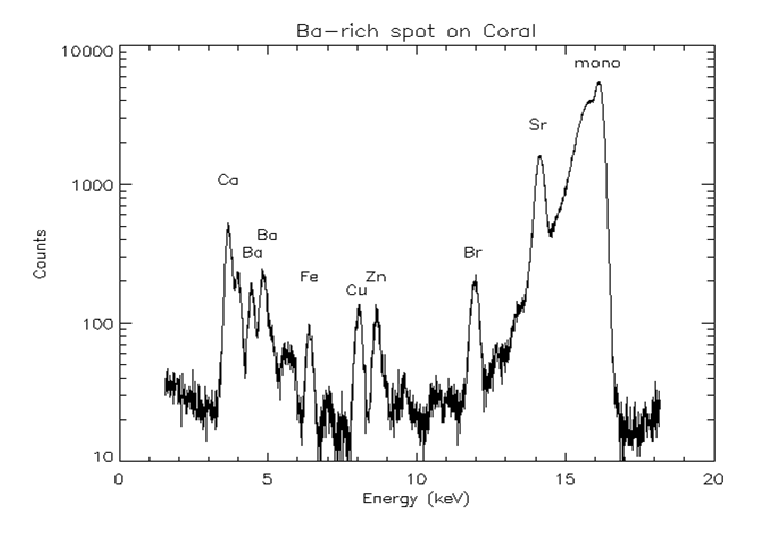
\includegraphics[width=53mm]{figs/general/xrf_spectra}
    \end{center}

  \end{minipage} 
  & 
  \begin{minipage}{53mm}
    {\tiny{
        \begin{entry}
      \pause
    \item[{\Red{Any Element}}]  $Z \gtrsim 4$, depending on source.
      \pause
    \item[{\Red{Element Specific}}]  can distinguish many elements in a
      compound.
      \pause  
    \item[{\Red{Fast Collection}}] Spectra can be collected in $\sim 1$ sec.
      \pause  
    \item[{\Red{Quantitative}}] Precise and Accurate Elemental abundances.
      \pause
    \item[{\Red{Low Concentrations}}] down to ppm levels, typically.
      \pause
    \item[{\Red{Minimal Sample Needs}}] natural samples, solutions,
      liquids, solids, soils, surfaces, etc.
    \end{entry}
  }}
\end{minipage} \\
\end{tabular}

\vmm\pause

XRF can be combined with other techniques and conditions: XRD, XAFS.

\vmm\pause 

With a synchrotron (or electron microscope), XRF can be used as a
{\RedEmph{microprobe}} for both quantitative elemental abundances and
XRF mapping  elemental distributions.

\vfill
\end{slide} 
